\documentclass{article}
\usepackage[utf8]{inputenc}
\usepackage[margin = 0.8in]{geometry}
\usepackage{graphicx}
\usepackage{amsmath, amssymb}
\usepackage{caption}
\usepackage{subcaption}
\usepackage{multirow}
\usepackage{multicol}
\usepackage{booktabs}
\usepackage{bm}
\setlength{\columnsep}{.75cm}
\usepackage{float}
\usepackage{graphicx}
\usepackage{stfloats}
\graphicspath{ {./images/} }
\setcounter{MaxMatrixCols}{15}

%\usepackage[parfill]{parskip}. %to not indent paragraph
\renewcommand\refname{References}
\restylefloat{table}


\title{LQR Control of a Nonlinear Quadrotor System}
\author{Keith Chester, Bob DeMont, Sean Hart}
\date{November 9th, 2021}

\begin{document}

\maketitle

\begin{figure}[h]
    \centering
    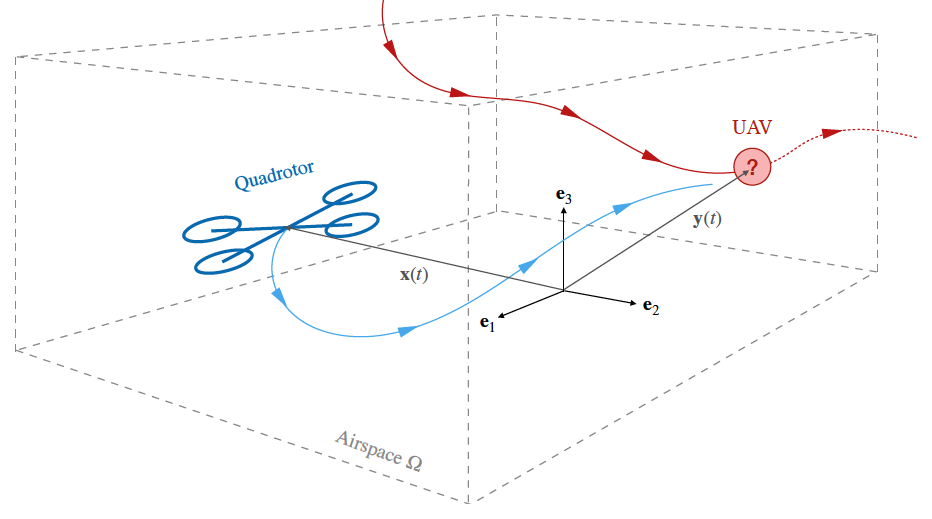
\includegraphics[width =0.75\textwidth]{images/ProjProbStmt.png}
    \label{fig:prob}
\end{figure}

\begin{multicols}{2}


\section*{Abstract}

The purpose of the project is to simulate the control and stable flight of an unmanned four rotor flying vehicle known as a quadrotor.  The problem is set into three goals: simulate and control the quadrotor hover in a stable configuration, chase an interloping quadrotor in flight and intercept, and return with the captured target quadrotor with randomized disturbance force while maintaining stable flight.

\section*{Situation/Problem}
The mission is defense of a designated airspace.  Our quadrotor is assigned to monitor a limited airspace, launch if an unidentified UAV enters that airspace, capture the target, and return to base.  If the target leaves the airspace before being captured, our quadrotor should return to base.  When captured, the target should be assumed to generate external forces on our UAV. The figure on the title page depicts the scenario.


\section*{Setup}

\noindent Coordinate frames are identified for the reference/inertial frame $E={e_1, e_2, e_3}$ at the center bottom of the airspace and the body frame $C={c_1, c_2, c_3}$.  All rotors are equidistant from the center of mass and in the same $c_1-c_2 $ plane as the body center of mass.  The external forces and moments on the system are represented by $\boldsymbol{r}$ and $\boldsymbol{n}$, where $\boldsymbol{r} = r_1 c_1 + r_2 c_2 + r_3 c_3$ and $\boldsymbol{n} = n_1 c_1 + n_2 c_2 + n_3 c_3$ directly applied to the center of mass. We are assuming that the torque of the rotor is proportionaly related to the input thrust via the constant $\sigma>0$, for $\tau_i = \sigma u_i$. We will be utilizing $\boldsymbol{I}$ as our diagonal inertial matrix where diagonal elements  $I_x, I_y $ and $I_z$ represent the mass moments of inertia about $c_1, c_2 $ and $c_3$ respectively.  For the purpose of our analysis we'll ignore the drag. The parameters for our state are described in table $\ref{table:Qparams}$.


\begin{table*}[t] %[bp]
\begin{centering}
\begin{tabular}{|cccc|}
\hline
Parameter & Value & Units  & Description  \\
\hline
 $l$  &  .02& m & Distance from center of mass to center of each rotor  \\
 $m$& .5 & kg &Total mass of quadrotor   \\
 $I_{x}$ & 1.24 kgm$^2 $ & s  & Mass moment of inertia about $c_1$ axis \\
 $I_{y}$ & 1.24 kgm$^2 $ & s  & Mass moment of inertia about $c_2$ axis \\
 $I_{z}$ & 1.24 kgm$^2 $ & s  & Mass moment of inertia about $c_3$ axis \\
$ g$ &9.81 & m/s$^2$ & Gravitational acceleration\\
$\sigma\ $& .01 & m & Proportionality constant relating $u_i $ to $\tau_i$\\
\hline
\end{tabular}
\caption{Quadrotor Parameters}
\label{table:Qparams}
\end{centering}
\end{table*}


\section*{General Approach}
We'll begin by generating the state space variables and defining the state space.  We'll prove controllability of the system and choose a controller methodology.  Using the controller, we will simulate hover as well as move to location and hover.  Finally we'll introduce external forces and moments that would be experienced simulating a target capture in the problem statement.  For ease of variable passing, our quadcopter will be represented as a structure in Matlab, with full state variables, A and B matrices, K gain matrix, $K_{capture}$ gain matrix (incorporating $n$ and $r$ forces and torques from the target) as well as characteristics for graphing (colors etc).

\section*{Methods}
We'll establish the state variable, $\mathbf{z}$ to represent the quadrotor's xyz center-of-mass position in the earth 
frame $\mathbf{x}=[x_1, x_2, x_3]$; the roll, pitch, yaw angles in the earth frame, $\bm{\alpha}=[\phi,\theta\psi]$; the xyz linear velocities in the earth frame, $\mathbf{v}=[v_1, v_2, v_3]$; and the angular accelerations $\bm{\omega}=[\omega_1, \omega_2, \omega_3]$ in the earth roll pitch yaw directions. Our state variable then is $\mathbf{z}=[\mathbf{x},\bm{\alpha},\mathbf{v},\bm{\omega}]^T$ and our state space is defined as:

\begin{equation}
    \mathbf{\dot{x}} =\mathbf{v}
\end{equation}
\begin{equation}
    \bm{\dot{\alpha}} =\mathbf{T}^{-1}\bm{\omega}
\end{equation}
\begin{align}
    \mathbf{\dot{v}} =-ge_3+\frac{1}{m}\mathbf{R_{C/E}}(u_1+u_2+u_3+u_4)c_3 \nonumber\\ +\frac{1}{m}\mathbf{R_{C/E}}r
\end{align}
\begin{align}
    \bm{\dot{\omega}} =I^{-1}((u_2-u_4)lc_1+(u_3-u_1)lc_2 \nonumber\\ +(u_1-u_2+u_3-u_4)\sigma c_3+n-\omega \times I \omega)
\end{align}

\noindent ...where $\mathbf{R_{C/E}}$ is defined in the problem statement as the Euler rotation matrix from quadrotor frame $C$ to earth frame $E$ and $\mathbf{T}^{-1}$, also defined in the problem statement, relates the angular rate of change of the Euler angles based on the angular velocity of the quadrotor.
%Equation development commented out
%\begin{equation}
%    \mathbf{R_{C/E}}=
%    \begin{bmatrix}
%        \cos \left(\psi \right)\,\cos \left(\theta \right) & \cos \left(\psi \right)\,\sin \left(\phi \right)\,\sin \left(\theta \right)-\cos \left(\phi \right)\,\sin \left(\psi \right) & \sin \left(\phi \right)\,\sin \left(\psi \right)+\cos \left(\phi \right)\,\cos \left(\psi \right)\,\sin \left(\theta \right)\\
%        \cos \left(\theta \right)\,\sin \left(\psi \right) & \cos \left(\phi \right)\,\cos \left(\psi \right)+\sin \left(\phi \right)\,\sin \left(\psi \right)\,\sin \left(\theta \right) & \cos \left(\phi \right)\,\sin \left(\psi \right)\,\sin \left(\theta \right)-\cos \left(\psi \right)\,\sin \left(\phi \right)\\
%        -\sin \left(\theta \right) & \cos \left(\theta \right)\,\sin \left(\phi \right) & \cos \left(\phi \right)\,\cos \left(\theta \right)
%    \end{bmatrix}
%\end{equation}
%And 
%\begin{equation}
 %   \mathbf{T}^{-1} = \begin{bmatrix}
 %       1 & \sin{\phi} \tan{\theta} & \cos{\phi}\tan{\theta} \\
 %       0 & \cos{\phi} & -\sin{\phi} \\
 %       0 & \frac{\sin{\phi}}{\cos{\theta}} & \frac{\cos{\phi}}{\theta}
  %  \end{bmatrix}
%\end{equation}

Our system is nonlinear because it is under-actuated; four actuators for six degrees of freedom. We can approximate its behavior using linear approximation.  We can then derive  our $\boldsymbol{K}$ matrix to determine our control.  We desire to get it into the linear format $\dot{x} = Ax + Bu$.
\noindent For a linearization in the neighborhood of a desired state space we'll define error $ e :=  z_d-z $ and change our inputs to $ w :=  u_d-u $.
With $u_d$ being the input to obtain the desired  state variable $z_d $.  We obtain the linearization through Taylor series expansion around the desired $(z_d,u_d)$

%which is generally 
%\begin{align}
%	\begin{split}
%f(z,u)&\approx f(z_d,u_d)+\frac{\delta f}{\delta z}\bigg \vert_{(z_,u)=(z_d,u_d)}(z-z_d)+\frac{\delta f}{\delta u}\bigg \vert_{(z_,u)=(z_d,u_d)}(u-u_d) 
%	\end{split}
%\end{align}
%With our $f(z,u)$
%\begin{gather}
%f(z,u)=
%\begin{bmatrix}
%v_1 \\
%v_2 \\
%v_3 \\
%\omega_1 +\omega_3 \cos\phi\tan\theta+\omega_2 \sin\phi\tan\theta \\
%\omega_2 \cos\phi -\omega_3 \sin \phi\\
%\frac{\omega_3 \cos\phi +\omega_2 \sin \phi }{\cos\theta}\\
%\frac{\sin \phi\sin\psi +\cos\phi \cos \psi \sin\theta (u_1 +u_2 +u_3 +u_4 )}{m}\\
%-\frac{\cos\psi\sin \phi-\cos\phi \sin \psi\sin \theta(u_1 +u_2 +u_3 +u_4 )}{m}\\
%\frac{\cos\phi\cos\theta(u_1 +u_2 +u_3 +u_4 )}{m}-g\\
%\frac{l(u_2 -u_4 )+I_y \omega_2 \omega_3 -I_z \omega_2 \omega_3 }{I_x }\\
%-\frac{l(u_1 -u_3 )+I_x \omega_1 \omega_3 -I_z \omega_1\omega_3 }{I_y }\\
%\frac{\sigma(u_1 -u_2 +u_3 -u_4 +I_x \omega_1 \omega_2 -I_y \omega_1 \omega_2 }{I_z }
%\end{bmatrix}
%\end{gather}
Taking the derivative of our error function $\dot{e}=\dot{z}_d-\dot{z}$ and substituting %(and pulling out the negative so that in the next step $z-z_d=-e$ and $u-u_d=-w$):
%\begin{equation}
%\dot{e}\approx f(z_d,u_d)-f(z_d,u_d)- f(z_d,u_d)+\frac{\delta f}{\delta z}\bigg %\vert_{(z_,u)=(z_d,u_d)}(z_d-z)+\frac{\delta f}{\delta u}\bigg \vert_{(z_,u)=(z_d,u_d)}(u_d-u) 
%\end{equation}
%The first two terms cancel, and substituting for our positional error $(z-z_d)=e$ and input $(u-u_d)=w$
%\begin{gather}
%	\dot{e}\approx
%	\begin{bmatrix}
%		0 & 0 & 0 & 0 & 0 & 0 & 1 & 0 & 0 & 0 & 0 & 0\\
%		0 & 0 & 0 & 0 & 0 & 0 & 0 & 1 & 0 & 0 & 0 & 0\\
%		0 & 0 & 0 & 0 & 0 & 0 & 0 & 0 & 1 & 0 & 0 & 0\\
%		0 & 0 & 0 & 0 & 0 & 0 & 0 & 0 & 0 & 1 & 0 & 0\\
%		0 & 0 & 0 & 0 & 0 & 0 & 0 & 0 & 0 & 0 & 1 & 0\\
%		0 & 0 & 0 & 0 & 0 & 0 & 0 & 0 & 0 & 0 & 0 & 1\\
%		0 & 0 & 0 & 0 & g & 0 & 0 & 0 & 0 & 0 & 0 & 0\\
%		0 & 0 & 0 & -g & 0 & 0 & 0 & 0 & 0 & 0 & 0 & 0\\
%		0 & 0 & 0 & 0 & 0 & 0 & 0 & 0 & 0 & 0 & 0 & 0\\
%		0 & 0 & 0 & 0 & 0 & 0 & 0 & 0 & 0 & 0 & 0 & 0\\
%		0 & 0 & 0 & 0 & 0 & 0 & 0 & 0 & 0 & 0 & 0 & 0\\
%		0 & 0 & 0 & 0 & 0 & 0 & 0 & 0 & 0 & 0 & 0 & 0
%	\end{bmatrix}
%	e
%	+
%	\begin{bmatrix}
%		0 & 0 & 0 & 0\\
%		0 & 0 & 0 & 0\\
%		0 & 0 & 0 & 0\\
%		0 & 0 & 0 & 0\\
%		0 & 0 & 0 & 0\\
%		0 & 0 & 0 & 0\\
%		0 & 0 & 0 & 0\\
%		0 & 0 & 0 & 0\\
%		\frac{1}{m} & \frac{1}{m} & \frac{1}{m} & \frac{1}{m}\\
%		0 & \frac{l}{I_x} & 0 & -\frac{l}{I_x}\\
%		\frac{l}{I_y} & 0 & -\frac{l}{I_x} & 0\\
%		\frac{\sigma}{I_z} & -\frac{\sigma}{I_z} & \frac{\sigma}{I_z} & -\frac{\sigma}{I_z}
%	\end{bmatrix}
%	w
%\end{gather}
allows us to obtain our \textbf{linear approximation of the system}  in the error dynamic written in the form $ \dot{e}=Ae+Bw$.
In order to make certain that our system is \emph{controllable}, we must ensure that the combinations of our state and input matrices are linearly independent to the degree that we have an independent column for each state.  To do so, we check rank of the controllability matrix assure that we have rank equal to the number of states in our z vector.  The controllability matrix is defined as:

\begin{equation}
C = \begin{bmatrix} B & AB & A^2B & A^3B & \dots & A^{10}B & A^{11}B\end{bmatrix}
\end{equation}

\noindent When we find the rank of our $C$ matrix, we find that the rank is as expected - 12. This confirms that the \textbf{system is controllable}. We can use the error dynamic equation$\dot{e} = (A - BK)e$  to determine the closed loop gain matrix K.

\section*{LQR Controller}
We selected the Linear-Quadratic Regulator (LQR) approach as an optimal control technique for generating the gain matrix, K.  LQR operates on the linearized system above utilizing both A matrix (states) and B matrix (inputs), and adds two matrices, Q and R which correspond to A and B and whose purpose is to impose a cost so the algorithm may trade off between the state and the actuators in the optimization.  Since we are not asked to weigh the cost of using the actuators (as if we were conserving fuel) , we have left the R matrix as a diagonal matrix of ones.  We have also not yet weighed the Q matrix, leaving it too as a matrix of diagonal ones, so that we may experiment in the future what is the best way to prioritize states in the system.  N is an interaction penalty matrix which will be assumed to not be relevant for this analysis.
\noindent
LQR acts on the linearized system of the form $\dot{x} = Ax + Bu$ and calculates a cost function based on optimization.  This integrates the costs of both Q and R for comparison :
\begin{equation}
J =x_0^TF(0)x(t_0) +  \int_{t_0}^{t_f} x^TQx+u^TRu +2x^TNu\,dt 
\end{equation}
\noindent
The control input u that minimizes this cost function is $u= -Kx$ with the K value is given by
\begin{equation}
K = R^{-1}(B^TP(t) + N^T)
\end{equation}
\noindent
Where P is created by solving Ricatti's continuous time differential equation:
\begin{equation}
A^TP(t) + P(t)A - (P(t)B + N)R^{-1}(B^TP(t) + N^T) + Q = \dot{P(t)}
\end{equation}
\noindent
and P(t) is bounded by $P(0) = F(0)$\\

\noindent The K is then used in our original, non linear system as the control function for the simulation.  
\bigskip
\section*{Modelling}

\noindent
The foundation of simulating the controller is the solution of the system of differential equations of our original system with the added gain from our LQR controller.  We have wrapped the changes in the environment into a separate function to serve as the ODE function in order to incorporate time-related changes to the target path as well as n and r forces and torques after capture.
\section*{Quadrotor Hovering}
To demonstrate successful control of our quadrotor, we establish an initial state of $z=[\mathbf{0}]$ and a desired state $z_d=[5,5,5,0,0,0,0,0,0,0,0,0] $ to demonstrate move and hover.  Feeding these into our ODE45 solver, we obtain smooth movement and hovering at the given $z_d$.  (Note initial and final states as well as trajectory plotted) in Figure 1.
\section*{Quadrotor Return to Base}
A mission objective was also to return to base if the target exits the envelope before capture.  Figure 1.b. demonstrates this performance. In this scenario the interceptor leaves the base to pursue the target, but the target exits the airspace envelope before the interceptor gets close enough to capture.

\section*{Quadrotor Interception of Target}
For modeling we will input a piecewise continuous function for the target so that we can include it in a single differentiation.  In earlier iterations, we input random continuous movements of the target which were only revealed to our quadcopter each second.  We resolved the ODE for new $z_d$ in a loop and were readily able to converge, so we believe the known "unknown" target trajectory to be an allowable simplification for solve time.\\
\\
For interception, it is assumed that the target is intercepted if we get within a distance of .3m of it.   Our simulation demonstrates successful interception of the target after tuning the Q matrix to de-emphasize errors in the z direction (to enable smooth up/down movement) and penalize x-y errors.  
\begin{figure}[H]
\centering
\begin{subfigure}[b]{0.31\textwidth}
    \centering
    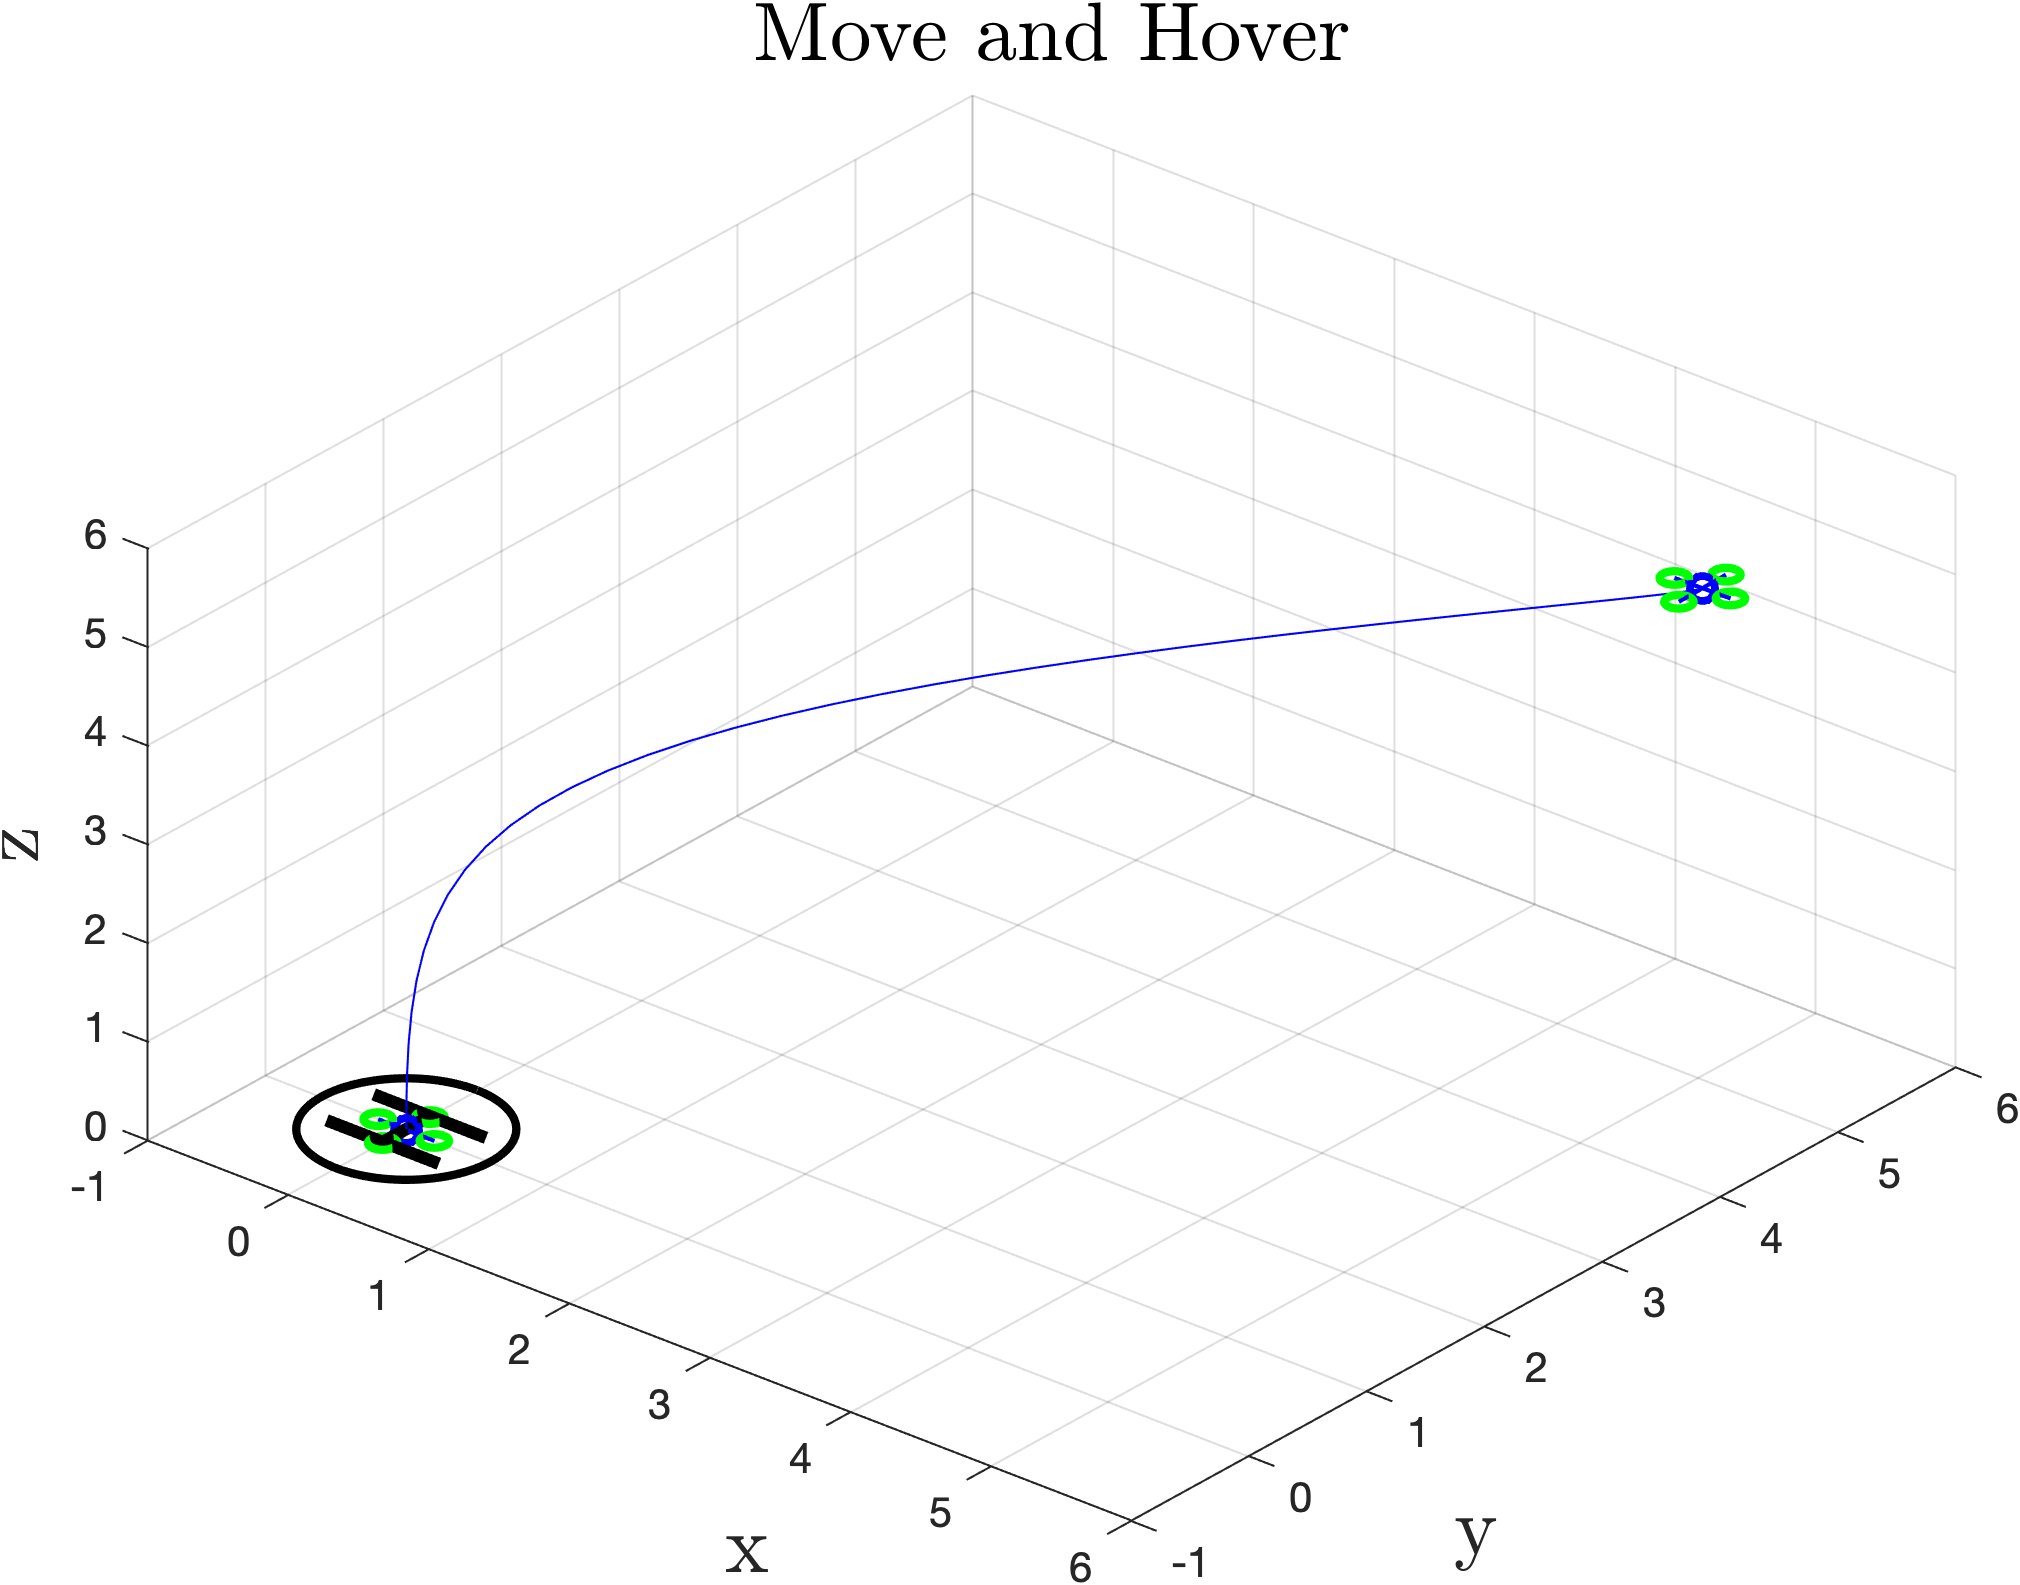
\includegraphics[width = 1\textwidth]{images/MoveAndHover.png}
     \label{fig:MandH}
     \caption{Quadrotor Move and Hover}
\end{subfigure}
\begin{subfigure}[b]{0.31\textwidth}
    \centering
    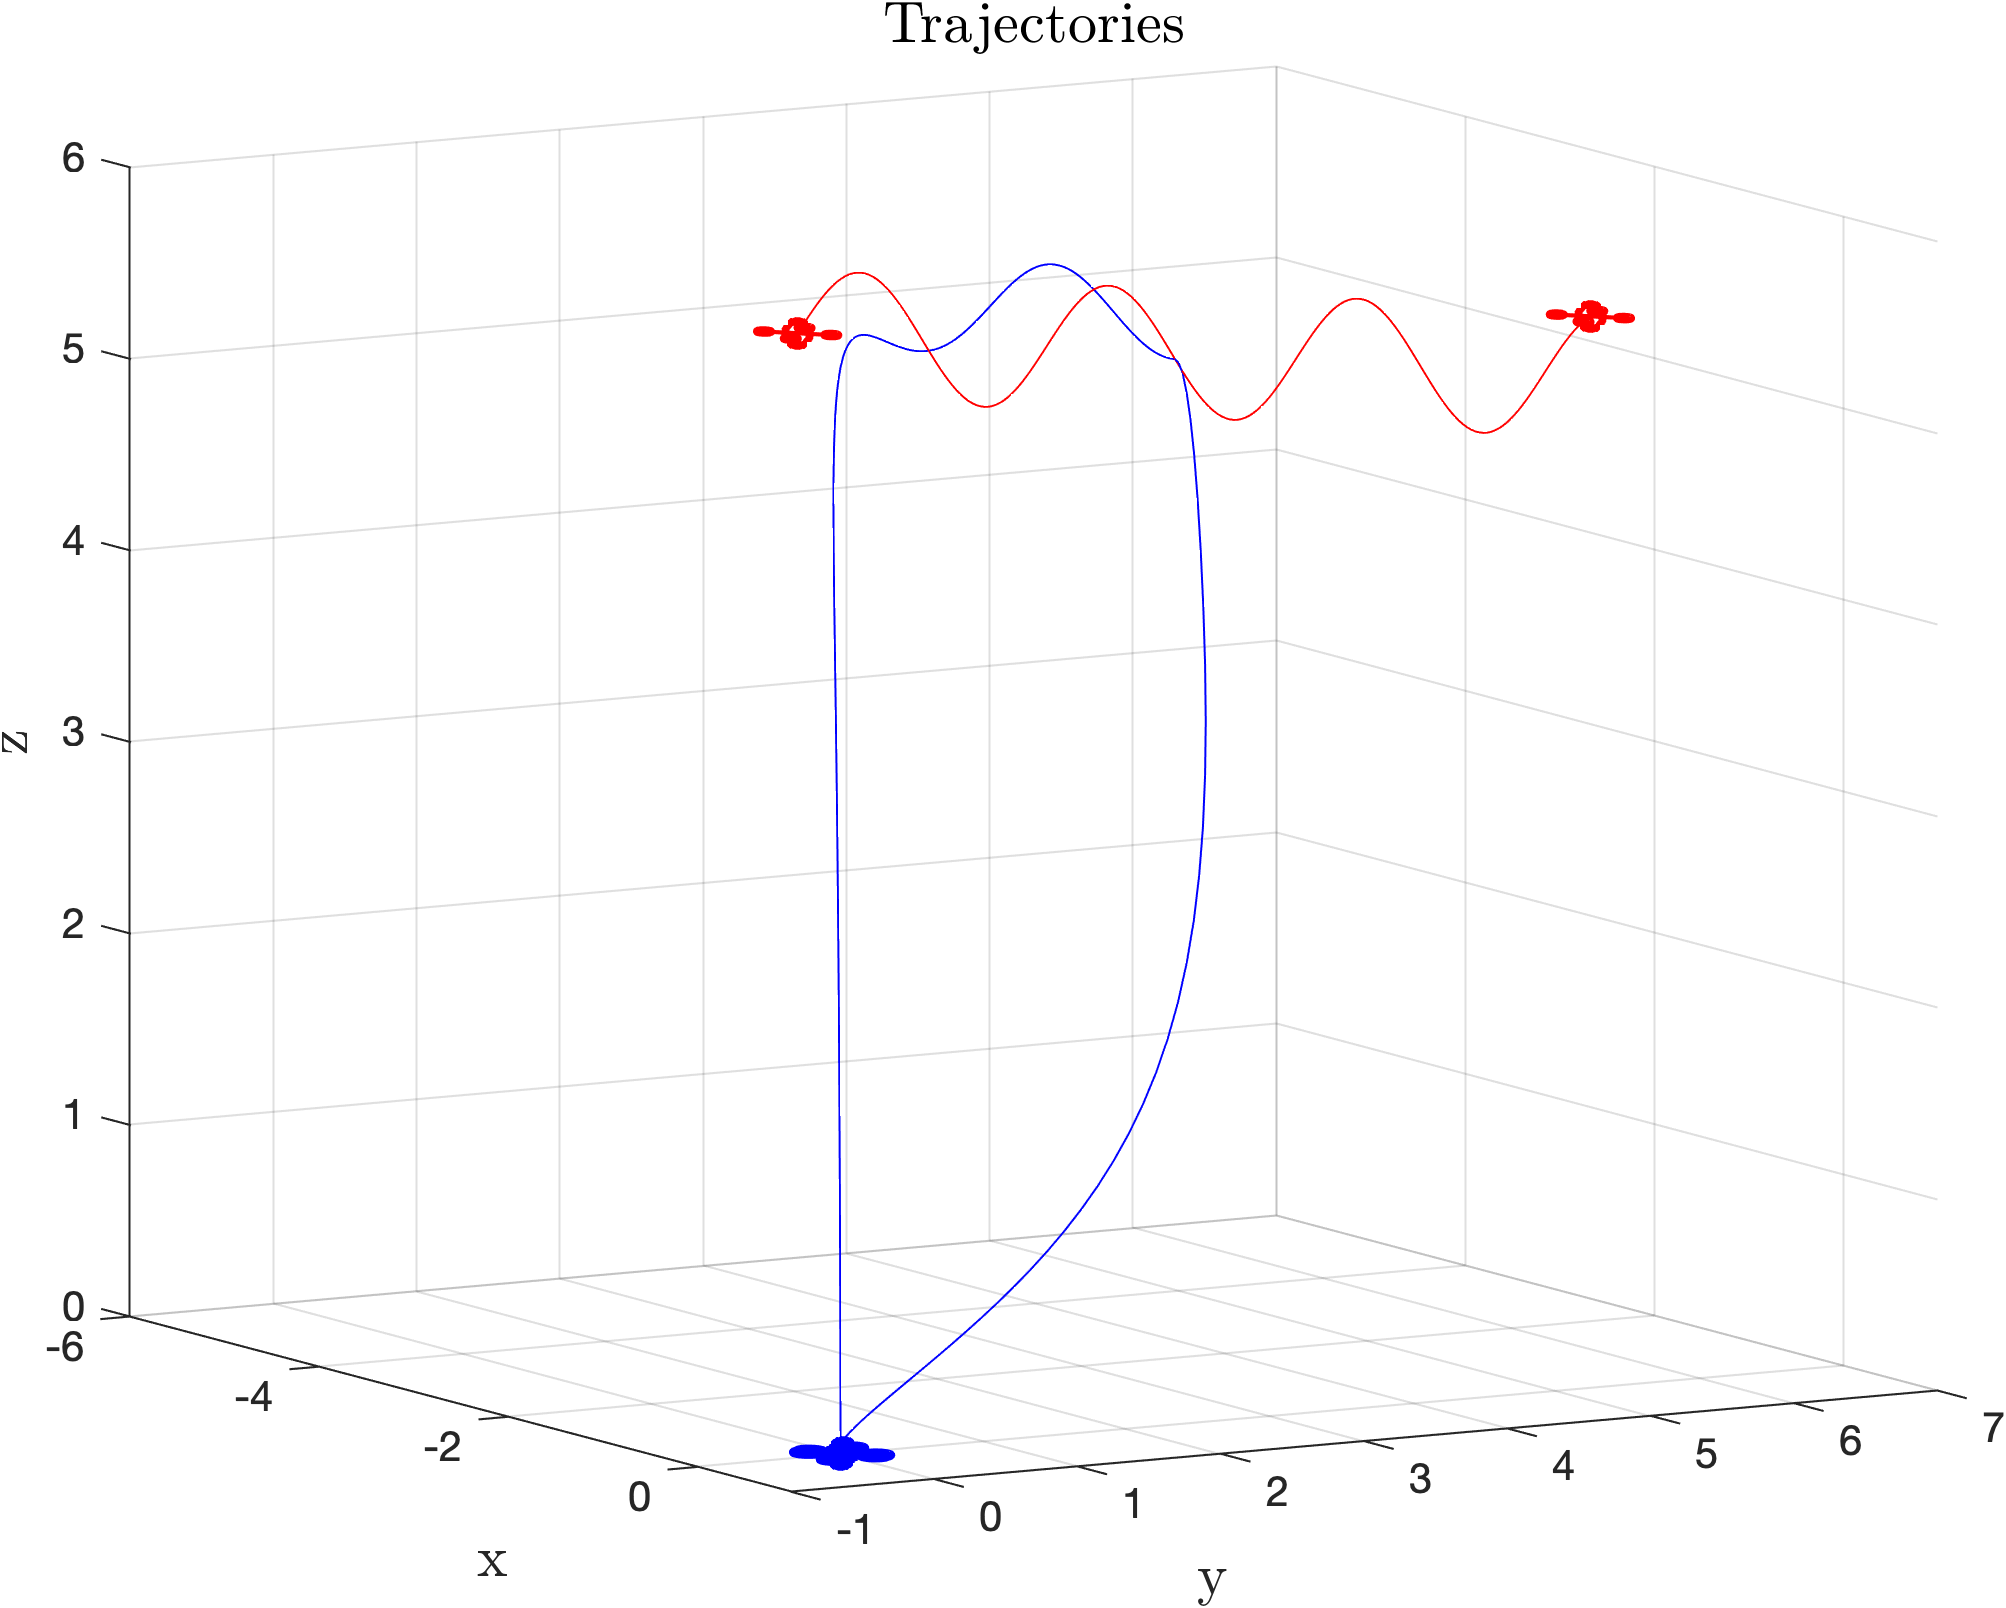
\includegraphics[width = 1\textwidth]{images/ReturnToBase.png}
     \label{fig:Return}
     \caption{Return to Base}
 \end{subfigure}
\begin{subfigure}[b]{0.31\textwidth}
    \centering
    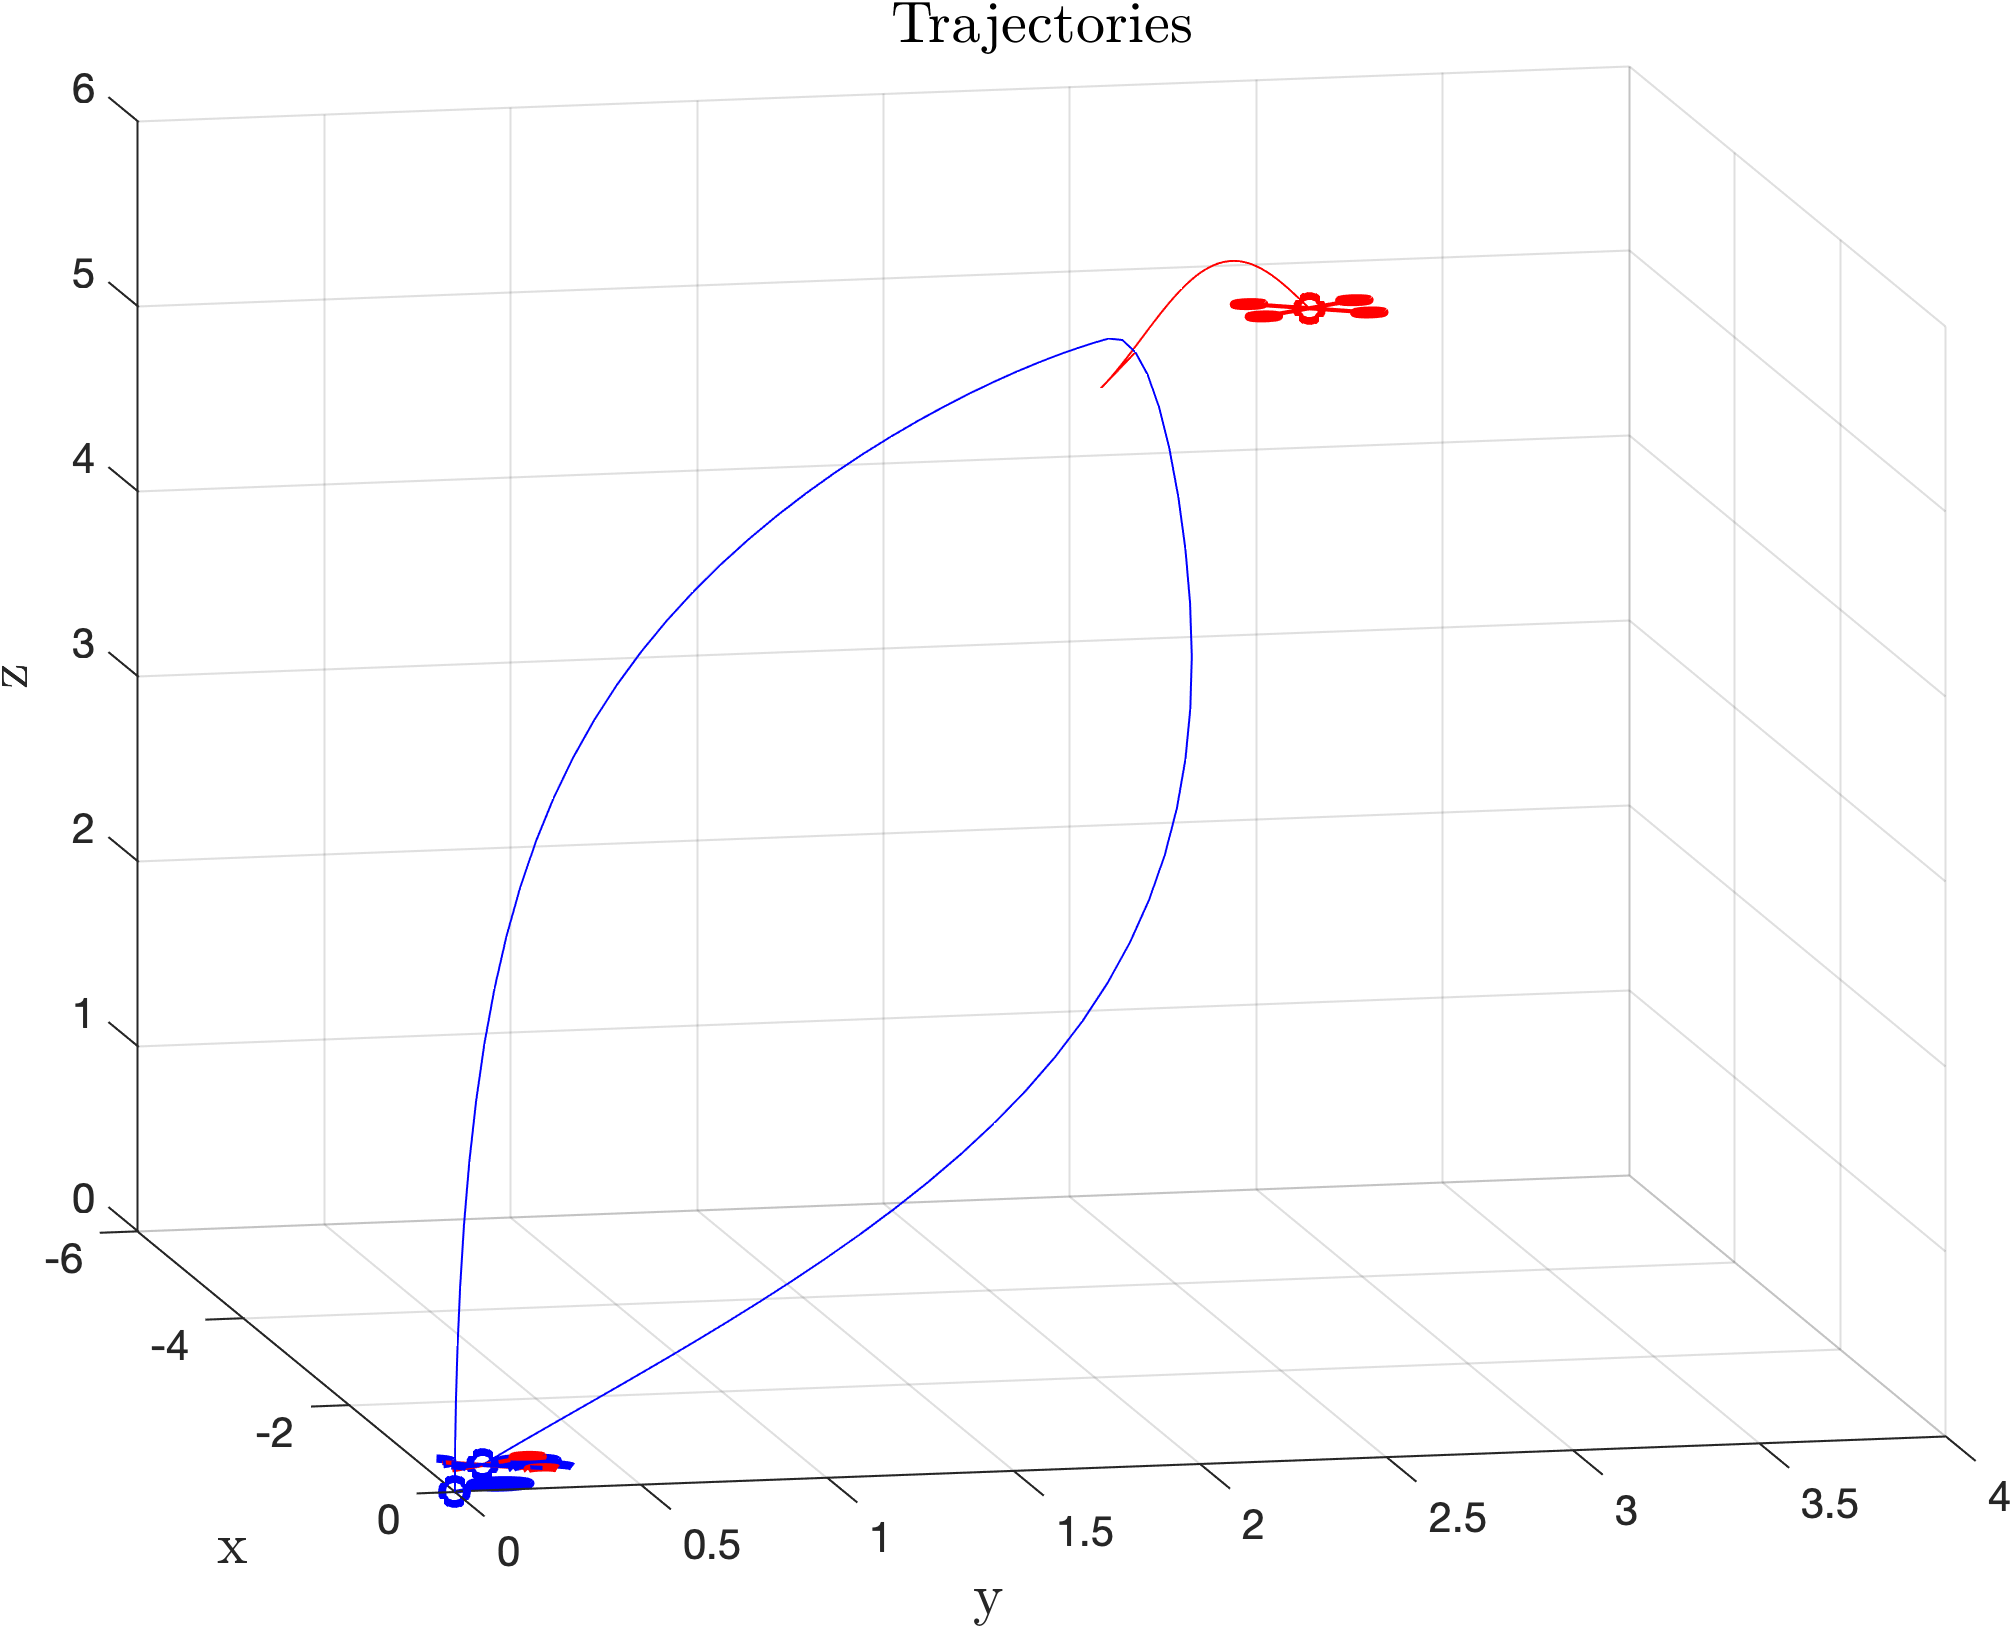
\includegraphics[width = 1\textwidth]{images/Intercept.png}
     \label{fig:Capture}
     \caption{Quadrotor Capture}
 \end{subfigure}
   \caption{Quadrotor Performance Tests}
\end{figure}

\bigskip
\section*{Quadrotor Return to Base with a Disturbance Force}
For the disturbance forces and torques after capture,  in the control of the ODE function we trigger an change in $n$ and $r$ and re-evaluate K before adding the mass of the target drone to recalculate the control, $u$, term for the ODE.  Again we use the simplification of a time dependent function for the $n$ term $n=[\sin(t)/10; \cos(t)/10; \sin(t)/10]$ to simulate the target trying to escape.  Where the terms of $n$ are in the order of 1/10 $\sin$ and $\cos$ the interceptor handles the torque well.  On the order of 1/5, initial movements after capture are handled well, but as the interceptor slows to land it has more trouble maintaining control.  At a full 2N torque(represented as 1/1) the system becomes unstable. Between 1/5 and 1/1, the interceptor combination returns close to base but crashes before reaching coordianates (0,0) in the (x,y) even with greater penalties in the $z$ section of the Q matrix.\\
  
\textbf{(End current edits)}
\section*{Results}
\section*{Discussion}

\label{References}
\bibliographystyle{abbrv}
\begin{thebibliography}{10}
\bibitem{JKim}
Jinho Kim, S. Andrew Gadsden, Stephen A . Wilkerson.
"A Comprehensive Survey of Control Strategies for Autonomus Quadrotors".
arXiv:2005.09858v1.
20 May 2020.
\bibitem{AHM}
Faraz Ahmad, Pushpendra Kumar, Anamika Bhandari, Pravin P. Patil.
Simulation of the Quadrotor Dynamics with LQR based Control.
Materials Today: Proceedings,Volume 24, Part 2, 2020, Pages 326-332,
ISSN 2214-7853.
https://doi.org/10.1016/j.matpr.2020.04.282.
\bibitem{OKY}
Okyere, E., Bousbaine, A., Poyi, G. T., Joseph, A. K., and Andrade.,
J. M. (2018) ‘LQR controller design for quad-rotor helicopters’,
The 9th International Conference on Power Electronics, Machines
and Drives. The Arena and Convention Centre, Liverpool, 17-19
April. London: The Institute of Engineering and Technology, pp.1-7
\bibitem{SUI}
Suicez, Emre Can.  Trajectory Tracking of a Quadrotor Unmanned Aerial Vehicle (UAV) via Attitude and Position Control.  Thesis for MS in Aerospace Engineering.  Middle East Technical University. July 2014. Pages 57-58.
\bibitem{Mart}
Luís Martins, Carlos Cardeira, Paulo Oliveira,
Linear Quadratic Regulator for Trajectory Tracking of a Quadrotor,
IFAC-PapersOnLine,
Volume 52, Issue 12, 2019,Pages 176-181,ISSN 2405-8963,
https://doi.org/10.1016/j.ifacol.2019.11.195.
\bibitem{kon}
Kong, Chuin-Wei.  2021, May 25. Title of video Quadcopter Simulation and Control-LQR Controller. YouTube. https://www.youtube.com/watch?v=oixM0DKNMGM
\bibitem{AHM}
Abbot, Jake. 2012, April 7. LQR Method. YouTube. https://www.youtube.com/watch?v=St5L-ekOKGA
\bibitem{MLT}
Matlab Tech Talks. 2019, February 5. Optimal Control LQR. YouTube. https://www.youtube.com/watch?v=


\end{thebibliography}

\end{multicols}

\end{document}